\section{Introduction}
\begin{figure}
\centering
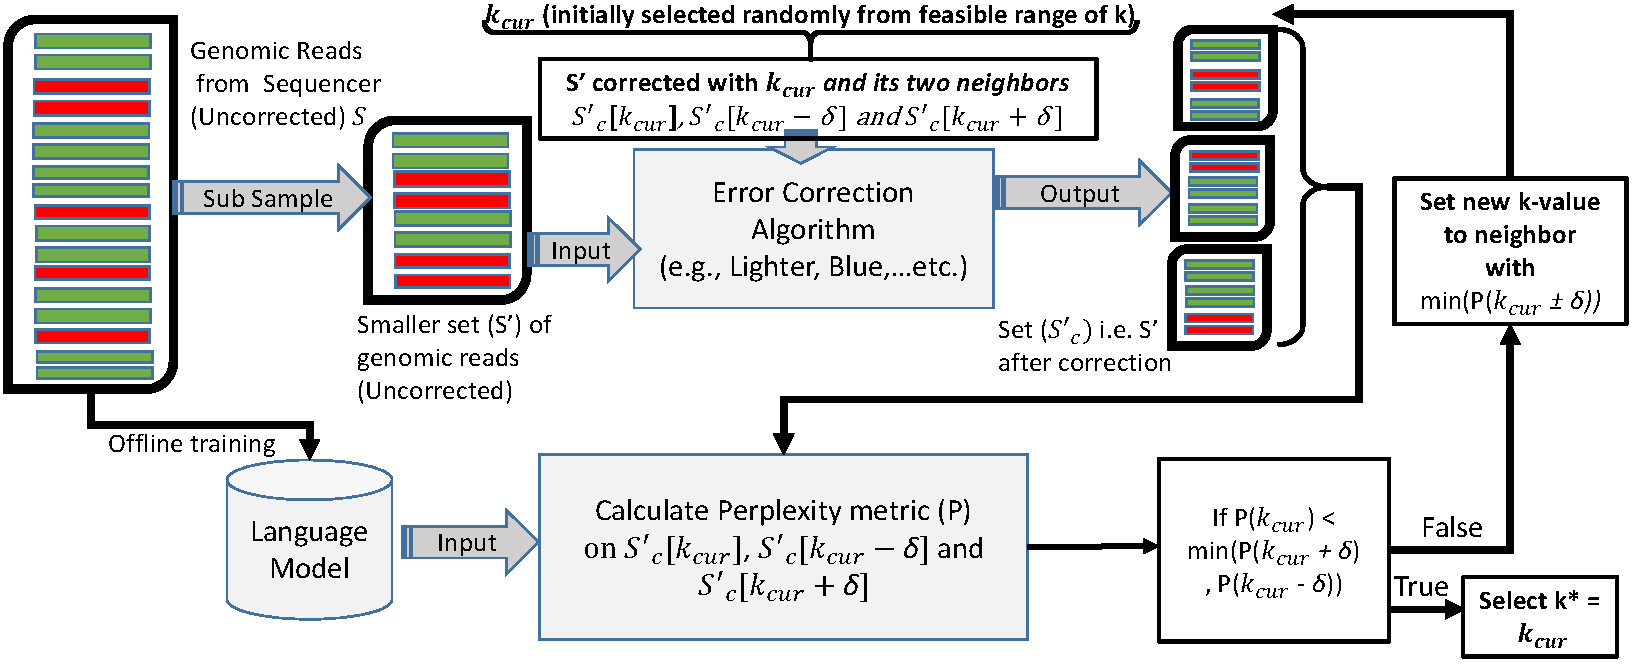
\includegraphics[width=\linewidth]{figs/AthenaOverview_Compressed2_cropped.pdf}
\caption{Overview of \name's workflow. First, we train the language model using the entire set of uncorrected reads for the specific dataset. Second, we perform error correction on a sub-sample from the uncorrected reads using an EC tool (\eg Lighter or Blue) and a range of $k$-values. Third, we evaluate the perplexity of each corrected sample and decide on the best $k$-value for the next iteration, \ie the one corresponding to the lowest perplexity metric because error correction quality is negatively correlated with the perplexity metric. This process continues until the termination criteria are met. Finally, the complete set of reads is corrected with the best $k$-value found.}	
\label{fig:AthenaOverview}
\end{figure}
\vspace{-10pt}
Rapid advances in genome sequencing technologies, with the resulting drops in sequencing costs, offer unprecedented opportunities to characterize genomes across the tree of life. %The first sequencing of the human whole genome (in 2003) cost roughly \$2.7 billion, reducing to the current thousand dollar regime, and further aspirations by Illumina to sequence the whole genome for less than \$100. This sharp drop in sequencing and operational costs is being fueled by the surge in powerful computing machines and optimized laboratory and computational processing techniques in recent years. 
While next-generation sequencing (NGS) techniques allow for rapid parallel sequencing vis-$\grave{a}$-vis older methods, NGS reads are more error-prone, especially for more complex genomes. %with exact or almost-exact repeat regions. 
In addition, sequencing platforms generate reads with different error profiles, including incorrect base replacements, insertions, deletions, etc. The current bottleneck of NGS projects is not the DNA sequencing process itself but the structured data management and sophisticated computational analysis downstream \cite{schadt2010computational}. In order to get biologically meaningful results, each step of the analysis workflow needs to be analyzed so errors are not magnified along the analysis pipeline.
% differing in size or copy number.
% SB (1/27/18): It may be better to talk of ``next generation sequencing'' than ``shotgun sequencing'' since our solution is even more applicable there. 
Consequently, multiple error-correction (EC) techniques have been developed to correct NGS reads in order to improve downstream applications, \eg, genome assembly \cite{mahadik2017scalable}, variant calling, and iterative k-mer selection for long-read error correction \cite{szalay2015novo, sameith2016iterative}. 
%Genomic read correction is computationally expensive, especially for short-read sequencing ($\leq$ 100-bp long), requiring high sequencing coverage, and with common applications in metagenomics and meta-transcriptomics \cite{meyer2017mg,chaterji2017federation}.

% SB (11/3/18): Why is EC expensive for short-read sequencing? I think the relevant factor is how many base pairs are in the read set. So if we have short-read sequencing and high coverage, that leads to large number of base pairs and hence short-read sequencing in expensive then. But it does not have to do with short-read sequency per se.
% Mus(11/3/18): You are right, Statement is not generally correct.
% SB (11/3/18): I do not understand the relevance of the part ``and with common applications ...''.
The performance of many EC algorithms is highly dependent on the proper choice of configuration parameters, such as the value of $k$ (length of the substring) in \textit{k}-spectrum-based techniques \cite{mahadik2017scalable}, where the original genomic reads are split into overlapping sub-strings of size $k$. By extracting these $k$-mers from sequenced reads, an efficient \textit{de Bruijn} Graph (DBG) \cite{compeau2011apply} can be built for genome assembly. Selecting different values of $k$ has a trade-off. Having small values of $k$ increases the overlap probability between reads. However, an unsuitably small value of $k$ degrades the EC performance because it does not allow the algorithm to discriminate between correct and erroneous $k$-mers. On the other hand, having unsuitably high $k$-values decreases the overlap probability and hurts EC performance \cite{sameith2016iterative}. This is because most $k$-mers will appear unique and thus not allow us to distinguish legitimate and erroneous $k$-mers. 
The $k$-mers that appear above a certain threshold frequency, and are therefore expected to be legitimate, are called \textit{solid k-mers}. The others are called \textit{insolid or untrusted $k$-mers}. (In $k$-spectrum-based methods, the goal is to convert insolid $k$-mers to solid ones with a minimum number of edit operations.) Both increasing or decreasing the overlap probability affects the EC capability and hence, there is an optimum value of $k$ to use. Further, this value changes with the dataset or the organism whose genome is being sequenced \cite{heydari2017evaluation}. Moreover, most EC tools are evaluated based on their direct ability on reducing error rates rather than improving the genome assembly \cite{heydari2017evaluation}. Although the assembly can benefit substantially from EC tools, miscorrected reads can often result in degraded assemblies from formation of incorrect chimera etc. \cite{heydari2017evaluation}.
% SB (11/3/18): The above sentence should be made more general - good EC can benefit all these applications - assembly and name others too. ``Formation of incorrect chimera'' is too specific and can be dropped. 
%\SCcomment{can sub-optimal values of k result in miscorrected errors? if so, show the plot you have a miscorrected read resulting in worse assembly than the uncorrected read.}
%\AMcomment{Added a citation}
% Consequently, 
%In our paper, we show that \name can automatically find the best values of k-mer sizes for a given dataset which improves the quality of the generated assemblies. % For example, authors in KmerGenie \CITE{chikhi2013informed} found that $k=61$ for the human chromosome 14 ``chr14'' data set improves the quality of assembly by 35\% over using $k=51$. On the contrary, using $k=61$ with the  \textit{Bombus impatiens} ``\textit{B. impatiens}'' data set {\em reduces} the quality of assembly by 8.6\% over using $k=51$. Thus, the optimum $k$ value selection must be done for each data set.
%Another important factor is that the performance often degrades sharply with divergence of the $k$ value away from the optimal value. Thus, the optimal value of $k$ for the Velvet assembler with the ``chr14'' data set, when applied to the same assembler with the ``S.  aureus'' data set gives an assembly quality that is degraded by 75\%. 
%\SCcomment{data-driven method instead of saying automated?}
% Mus: Done.
Therefore, a data-driven  method for finding the best value of \textit{k} and other configuration parameters is needed for improved error correction, and subsequently, for superior genome alignment, genome assembly, variant calling, and other applications downstream.
% SB (11/3/18): Added alignment which we do evaluate. 
%Mus(11/3/18): Makes sense.
% \SCcomment{we don't evaluate genome assembly, so a little dicey to say this}.
%\AMcomment{Moreover, several EC tools depend on not a single, but a set of configuration parameters that control the quality of the correction process. For example, Reptile has five performance-sensitive parameters and our technique can optimize the values of multiple configuration parameters, with their dependencies.(CFC as we don't show any exp. with many configs}
%\SCcomment{\name can model dependencies, right?}\AMcomment{I don't think so}
% (e.g., gain). 
%SC(05/19/08): little bit of a stretch in that last part but it does not make sense to have those 2 sentences in there otherwise, making the claim above makes our technique shine though, so good to have.

%better word choice? I put automated (SC) 

% \begin{figure}
%   \includegraphics[width=\linewidth]{Figures/Kmer_Genie.eps}
%   \caption{Adapted from \cite{chikhi2013informed}: Best value of $k$ found by Kmer-genie for genome assembly for three data sets: \textit{S. aureus} (Velvet), chr14 (Velvet), and \textit{B.impatiens} (SOAPdenovo2)}
%   \label{fig:Best_K_Different_Data_Sets}
% \end{figure}

% SB (1/27/18): Why?  Give concrete proof that a good k value for one dataset (one organism?) can give a bad assembly for another dataset. This can be done by showing assembly quality is bad for one and good for another.  


% Sensitivity is a less stringent measure as it is equivalent to number of reads containing errors and  was classified as True Positive irrespective of whether they were accurately corrected or not.

% SB (1/27/18): Define sensitivity and gain in the figure caption. 

% \begin{figure*}%[!tpb]%figure1
% %\fboxsep=0pt\colorbox{gray}{\begin{minipage}[t]{235pt} \vbox to 100pt{\vfill\hbox to
% %235pt{\hfill\fontsize{24pt}{24pt}\selectfont FPO\hfill}\vfill}
% %\end{minipage}}
% \centerline{\includegraphicss[width=0.8\textwidth]{Figures/Athena_Overview.pdf}}
% \caption{Overview of Athena Workflow}
% \end{figure*}


Many existing EC solutions (\textit{e.g.}, Reptile \cite{yang2010reptile}, Quake \cite{kelley2010quake}, Lighter \cite{song2014lighter}, Blue \cite{greenfield2014blue}) require users to specify $k$. The best value is usually found by exploration over a range of $k$ values \cite{kao2011echo} and evaluating the performance metric--- \eg EC Gain, Alignment Rate, Accuracy, Recall, and Precision \cite{heydari2017evaluation}.
% The domain-specific parameter ``gain'' measures the percentage of errors effectively removed from the data set.
However, a reference genome is typically needed to serve as ground truth for evaluation, which makes this approach infeasible for \textit{de novo} sequencing tasks or where a high-quality reference genome is unavailable. 
%SC(05/21/18): do novo used likelihood-based metrics, so not accurately written above
% SB (5/21/18): But de novo does not need reference genome. Likelihood based metrics are calculated without taking recourse to a reference genome. 
To the best of our knowledge, existing tools leave the best parameter choice to the end user~\cite{peng2010idba, mahadik2017scalable}, while few others provide intuitive histograms or heuristics to assist in the decision process~\cite{chikhi2013informed}.
% SB (11/3/18): Add one or two more citations that provide such help. 
% Mus(11/3/18): To our knoweldge, Kmergnie is the one which provides help. Will check again.
Thus, the need for a data-driven method to select the optimal $k$-value is crucial. 
\SBcomment{Provide a motivating quantitative result - one value of k good for one dataset gives really bad result with another dataset.} \AMcomment{For example, we found that $k$=25 gives the best performance for D5 using Lighter. However, if the same value of $k$ was used for D1, the Gain drops from 96.3\% (with $k$ = 17) to 69.96\% (See table \ref{tb1:Lighter-Perplexity-vs-Alignment} in APPENDIX).}
Our solution, {\em \name}\footnote{Just as \textit{Athena} is the Greek Goddess of wisdom and a fierce warrior, we wish our technique to unearth the genomic codes underlying disease in a fearless war against maladies.} finds the best value of the configuration parameters
for correcting errors in genome sequencing, such as the value of $k$ in $k$-mer based methods. Further, \name does not require access to a reference genome to perform its function of determining the optimal parameter configuration\footnote{In our evaluation, we use Bowtie2 to perform alignment and then measure the alignment rate as the metric to evaluate our solution. But alignment is not needed for \name to work.}. 
% genome to compute the quality of the corrected reads, although we use Bowtie to align against the reference genome for evaluation.
This makes it much faster compared to existing \textit{de novo} assembly quality metrics such as CGAL \cite{rahman2013cgal} and ALE \cite{clark2013ale}.
% SB (11/3/18): I do not understand the above sentence. This seems like an apples-to-oranges comparison - we are doing error correction and you are comparing it to assembly. Also, what does it mean to be faster than a metric?
%Thus, \name improves the performance of the error correction phase, which also improves the quality of genome assembly approaches---\textit{de novo} and comparative (reference-based) genome assembly. %\AMcomment{Why making it faster improves the performance and quality of assembly?} SC-- no it does not.. I don't recall writing this.
%During comparative genome assembly, a reference genome from the same or a closely related species is used to map the assembly process by aligning the fragments being assembled. Using \name for comparative sequencing obviates the need to use this reference genome. 
In the case of \textit{de novo} assembly, \name takes advantage of the fact that NGS reads have the property of reasonably high coverage, 30X--150X coverage depth is commonplace. 
 % 100x-ish is considered "high coverage", e.g.: https://www.biostars.org/p/55994/
Because of this property, it is well known that the likelihood of correct overlaps for a given portion of the genome will outnumber the likelihood of erroneous ones \cite{yang2010reptile}.
\begin{figure*}
  \includegraphics[width=\linewidth]{figs/PPL_Example.eps}
  \caption{An example showing how the perplexity metric encodes errors in genomic reads. The read on the left is an erroneous read selected from dataset \#3 (D3), while the read on the right is the same read, after correction with Lighter. When using language modeling to compute the perplexity for both reads, we notice that the read on the right has a lower perplexity value (15.2), relative to the erroneous read (77.72), as the sequence of $k$-mers after correction has a higher probability of occurrence. Also notice that the probability of a sequence of $k$-mers depends on both their frequencies and their relative order in the read, which allows the perplexity metric to capture how likely it is to observe this $k$-mer given the neighboring $k$-mers in a given read.}
  \label{fig:PPL_Simple_Example}
\end{figure*}
%\vspace{-1pt}
Thus, we utilize this property to capture the underlying semantics of NGS reads such that the language model (LM) can learn the complexities of a language and can also predict future sequences (words or sentences) using information retrieved from prior sequences. This is integral to traditional NLP tasks such as speech recognition, machine translation, or text summaries. LM's goal is to learn a probability distribution over sequences of symbols and words,
in this case specialized to the dataset where genome error correction is to be done. 
% \textit{personalized} to a specific genome's ``language''.
Therefore, it can be used to identify words ($k$-mers here) that do not fit into the context of the language and thus contribute to a high value of the metric called {\em ``perplexity metric''}. This personalization is very beneficial to our problem because the LM then learns the patterns, obvious as well subtle, of the sequenced genome.

In our context, we use LM to estimate the probabilistic likelihood that some observed sequence is solid or insolid. We train an LM using the original dataset (with uncorrected reads), and then use this trained model to compute the perplexity metric when the EC tool is run with a specific configuration, \ie for specific values of its parameters. 
%Although the LM is trained on the uncorrected reads, it can still identify the correct sequences due to the high coverage and overlap between the reads.
% SB (11/3/18): I don't see the relevance of the above sentence. 
% Mus(11/3/18): Commented it.
We show empirically that the perplexity metric is inversely correlated to the quality of error correction.
Crucially, the perplexity metric evaluation does not require the computationally expensive alignment to a reference genome.
Through a stochastic optimization method, we evaluate the search space to pick the best value of the configuration parameter to guide EC, \eg $k$ in $k$-mer-based methods and the Genome Length (GL) in the RACER EC tool. 

\noindent{In summary, this paper makes the following contributions}. 
\vspace{-6pt}
\begin{enumerate}
\item \name develops a language modeling suite such that the perplexity metric and the error correction quality (evaluated via alignment against a reference genome) are inversely related. This allows \name to efficiently drive a search for the best configuration parameter values for any existing EC tool. 
  % For synthetic datasets, we systematically vary the complexity and error rates and profiles. 
  % \SCcomment{do we do this.. as in systematically vary all if the above? if not, modify as you see fit.}
  % SB (11/3/18): Done. 
\vspace{-8pt}

\item We compare and contrast two LM variants, N-gram LM with and RNN-based LM. Through this, we show that N-Gram modeling can be faster to train while char-RNN modeling operates at a finer, single-basepair granularity, providing similar accuracy with significantly lower memory footprint. 
% \SCcomment{quantify significant}.
This latter property will be beneficial for supporting multi-tenant analysis pipelines, such as in the world's leading metagenomics portal MG-RAST \cite{meyer2017mg}.
%\AMcomment{ Which is very benificial for supporting multi-users analysis pipelines such as MG-RAST [Cite XXX]}. %\SCcomment{what is the intuition for this and will faster or lower memory footprint be better for larger or more complex genomes, for example.. add a line to indicate that.}
\vspace{-8pt}

\item We apply \name to 3 EC tools: Lighter \cite{song2014lighter}, Blue \cite{greenfield2014blue}, and RACER \cite{ilie2013racer}. We show that \name was successful in finding either the best parameters ($k$ for Lighter and Blue, and $Genome Length$ for RACER) or parameters that perform within 0.27\% in overall alignment rate to the best values using exhaustive search against a reference genome. We compared the performance of \name with 5 different real datasets, with varied error rates and read lengths. %The best parameters found by \name performed within , compared to the best values using exhaustive search against a reference genome.
% SB (11/3/18): The two sentences above seem to contradict each other. If we find the best parameters (first sentence), how come we are only close in the alignment rate to the theoretical best (second sentence)? 

% AM (11/4/18): Done
\end{enumerate}

%SC(05/16/18): for the contributions above, we need to give some numbers, such as the performance numbers in terms of the perplexity metric for example. Quantifiable claims are important.


